%!TEX TS-program = xelatex
%!TEX encoding = UTF-8 Unicode

\documentclass[11pt]{extarticle}
% extarticle is like article but can handle 8pt, 9pt, 10pt, 11pt, 12pt, 14pt, 17pt, and 20pt text

\def \ititle {Joint Action and the Emergence of Mindreading}
\def \isubtitle {}
\def \iauthor {Stephen A. Butterfill}
\def \iemail{s.butterfill@warwick.ac.uk}
\date{}

%remove all section numbers
 \setcounter{secnumdepth}{0}

%for strikethrough
\usepackage[normalem]{ulem}

\input{$HOME/Documents/submissions/preamble_steve_handout}

\bibpunct{}{}{,}{s}{}{,}  %use superscript TICS style bib
%remove hanging indent for TICS style bib
%TODO doesnt work
\setlength{\bibhang}{0em}
%\setlength{\bibsep}{0.5em}


%itemize bullet should be dash
\renewcommand{\labelitemi}{$-$}

\begin{document}

\begin{multicols}{3}

\setlength\footnotesep{1em}


\bibliographystyle{newapa} %apalike

%\maketitle
%\tableofcontents



\

\begin{center}
{
\textbf{Joint Action and the Emergence of Mindreading}
\Large{Interacting Mindreaders}
}


%Stephen A. Butterfill

<s.butterfill@warwick.ac.uk>

\end{center}

Could an interacting mindreader be in a position to know things which she would be unable to know were she unable to interact with her targets?



\section{Ordinary 3$^{\textrm{\tiny rd}}$ person interpretation} 

Csibra \& Gergely's principle of rational action: `an action can be explained by a goal state if, and only if, it is seen as the most justifiable action towards that goal state that is available within the constraints of reality.'\citep{Csibra:1998cx,Csibra:2003jv}

%(Cf.\ Southgate et al's principle of efficiency:
%`goal attribution requires that agents expend the least possible amount of energy within their motor constraints to achieve a certain end.' \citep%[p.\ 1061]
%{Southgate:2008el})

%


These facts:
%
\begin{enumerate}
%
\item action $a$ is directed to some goal;
%
\item actions of $a$'s type are normally capable of being means of realising outcomes of $G$'s type in situations with the salient (to any concerned) features of this situation;
% 
\item no alternative type of action is both 
typically available to agents of this type 
and also 
such that actions of this type would be normally be significantly better* means of realising outcome $G$ in situations with the salient features of this situation;
%
\item the occurrence of outcome $G$ is typically desirable for agents of this type;
%
\end{enumerate}
%
\begin{enumerate}[resume]
\item there is no other outcome, $G'$, 
the occurrence of which would be at least comparably desirable for agents of this type 
and where (2) and (3) both hold of $G'$ and $a$
%
%where
%	the occurrence of $G'$ would be at least comparably desirable for agents of this type 
%%where
%%	$G$'s occurrence is not a means to $G'$'s nor conversely,
%and
%where  
%	(2) and (3) both hold of $G'$ and $a$
\end{enumerate}
%
may jointly constitute defeasible evidence for the conclusion that:
%
\begin{enumerate}[resume]
\item $G$ is a goal to which action $a$ is directed.
\end{enumerate}
%

{
\footnotesize
*An action of type $a'$ is a better means of realising outcome $G$ in a given situation than an action of type $a$ if, for instance, actions of type $a'$ normally involve less effort than actions of type $a$ 
in situations with the salient features of this situation 
and everything else is equal; 
or if, for example, actions of type $a'$ are normally more likely to realise outcome $G$ than actions of type $a$
in situations with the salient features of this situation 
and everything else is equal.
}

%\section{The problem of opaque means}
%Ordinary 3$^{\textrm{\tiny rd}}$ person interpretation may fail when it is not known which outcomes a behaviour is a means of bringing about, especially where a novel tool or communicative device is used.

\section{Your-goal-is-my-goal}
\begin{enumerate}
\item You are willing to engage in some joint action or other with me.
%(for example, because you have made eye contact with me while I was in the middle of attempting to do something).

\item I am not about to change the single goal to which my actions will be directed.

\end{enumerate}
%
Therefore:
%
\begin{enumerate}[resume]
%
\item A goal of your actions will be my goal, the goal I now envisage that my actions will be directed to.
\end{enumerate}
%

\section{Application}

`to understand pointing, the subject needs to understand more than the individual goal-directed behaviour. She needs to understand that ... the other attempts to communicate to her ...  and ... the communicative intention behind the gesture'\citep{Moll:2007gu}


\begin{center}
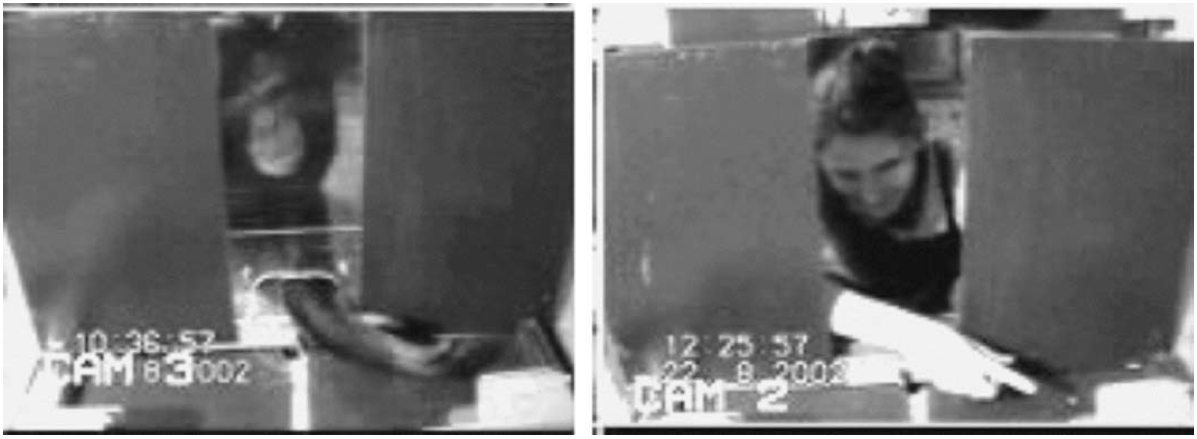
\includegraphics[width=6cm]{figure_hare_toma_2004_e3.png}
\label{fig:reach_point}

A failed reach (left) and a helpful point (right).\citep%[p.\ 557, figure 4]
	{hare_chimpanzees_2004}
\end{center}



`the adult’s social cues conveyed her communicative intent, which in turn encouraged the child to `see through the sign'.'
\citep%[p.\ 118]
{leekam_adults_2010}




\footnotesize 
\bibliography{$HOME/endnote/phd_biblio}

\end{multicols}

\end{document}